\section{Differentialgleichungen \formelbuch{543}}

\subsection{L"osen von Differentialgleichungen 1. Ordnung}

\subsubsection{Picard-Lindelöf}
Die Funktion $f\left(x, u, u_{1}, \ldots, u_{n-1}\right)$ sei in einer Umgebung der Stelle $\left(x_{0}, y_{0}, y_{1}, \ldots, y_{n-1}\right) \in \mathbf{R}^{\mathbf{n}+1}$ stetig und besitzt dort stetige partielle Ableitungen nach $u, u_{1}, \ldots, u_{n-1}$, dann existiert in einer geeigneten Umgebung des Anfangspunktes $x_{0}$ genau eine Lösung des Anfangswertproblems.\\
$y^{(n)}=f\left(x, y, y^{\prime}, \ldots, y^{(n-1)}\right)$ mit $y\left(x_{0}\right)=y_{0}, y^{\prime}\left(x_{0}\right)=y_{1}, \ldots, y^{(n-1)}\left(x_{0}\right)=y_{n-1}$\\
\newline
$\frac{\partial f(x,y,y,...)}{\partial y} \ldots \frac{\partial f}{\partial f^{(n-1)}}$ endlich beschränkt $\Rightarrow$ eindeutige Lösbarkeit

\subsubsection{Trennung von Variabeln / Separation \formelbuch{545}}
\begin{tabular}{p{4cm}p{1.5cm}p{10.5cm}}
\textbf{Form:} $y' = f(x) g(y)$ &
\textbf{Vorgehen:}              &
1. DGL umstellen: $\frac{y'}{g(y)} = f(x)$ \\ &&
2. Beidseitig nach x integrieren wobei $dx = \frac{dy}{y'}$ \\ &&
3. Genzen anpassen: $\int_{y_0=y(x_0)}^{y} \frac{1}{g(y)} dy =
\int_{x}^{x_0}f(x) dx$
\end{tabular}

\subsubsection{Lineartermsubstitution \formelbuch{545}}
\begin{tabular}{p{4cm}p{1.5cm}p{10.5cm}}
\textbf{Form:} $y'=f(ax+by+c)$   &
\textbf{Vorgehen:}               &
1. Substitution: $z=ax+by+c$ \\ &&
2. Einsetzen in $z^{\prime}=a+b y^{\prime}=a+b f(z)$\\ &&
3. Separation: $\int_{x_{0}}^{x} \frac{z^{\prime}}{a+b f(z)} d \tilde{x}=\int 1 d \tilde{x}$\\ &&
 $\Rightarrow \int_{z_{0}}^{z} \frac{1}{a+b f(\tilde{z})} d \tilde{z}=\int_{x_{0}}^{x} 1 d \tilde{x} \quad\left[d \tilde{z}=\underbrace{\left(a+b y^{\prime}\right)}_{z^{\prime}} d \tilde{x}\right]$
\end{tabular}

\subsubsection{Gleichgradigkeit}
\begin{tabular}{p{4cm}p{1.5cm}p{10.5cm}}
\textbf{Form:} $y'=f(\frac{y}{x})$ &
\textbf{Vorgehen:}                &
1. Substitution:\quad $z=\frac{y}{x}$\\ &&
2. Einsetzen in $z'=\frac{1}{x}(f(z)-z)$\\ &&
3. Seperation: $\frac{z'}{f(z)-z} = \frac{1}{x}$ wobei $z_0 = \frac{y_0}{x_0}$ 
\end{tabular}
\newline
\newline

\subsubsection{Lineare Differentialgleichungen 1. Ordnung \formelbuch{546}}
\begin{tabular}{p{4cm}p{1.5cm}p{10.5cm}}
\textbf{Form:} $ y'+f(x)y = g(x) $ &
\textbf{Vorgehen:}                 &
Homogene Rechunug: $y_H = k \cdot e^{-\int f(x) \cdot dx}$\\ &&
Inhomogene Rechunug: $y_P = (\int g(x) \cdot e^{\int f(x) \cdot dx} \cdot dx)
\cdot e^{-\int f(x) \cdot dx}$\\ &&
Allgemeine Lösung: $y = y_H + y_P$ wobei $k = \frac{y_0 - y_P(x_0)}{e^{\int
f(x_0) \cdot dx)}}$
\end{tabular}

\subsection{Lineare Differentialgleichung 2. Ordnung mit konstanten 
Koeffizienten \formelbuch{564}}
\begin{tabular}{p{8cm}p{8cm}}
\textbf{Form:} $y''+a_1\cdot y'+a_0\cdot y=f(x)$  &
\textbf{St"orglied:} $f(x)$\\
\textbf{Homogene Differentialgleichung:} $f(x)=0$ &
\textbf{Inhomogene Differentialgleichung:} $f(x)\neq 0$
\end{tabular}

\subsubsection{Allgemeine Lösung einer homogenen DGL:\quad $y=Y_H$}
\textbf{Charakteristisches Polynom} $\quad \lambda^{2}+a_{1} \cdot \lambda+a_{0}=0$\quad  von\quad $y^{\prime \prime}+a_{1} \cdot y^{\prime}+a_{0} \cdot y=0$\quad $\left(\lambda_{1,2}=-\frac{a_{1}}{2} \pm \frac{\sqrt{a_{1}^{2}-4 a_{0}}}{2}\right)$

$\begin{array}{lllll}
{\text{2 Lösungen}} & {(D>0)} & {\text { Falls } \lambda_{1} \neq \lambda_{2} \text { und } \lambda_{1,2} \in R :} & {Y_{H}=A e^{\lambda_{1} x}+B e^{\lambda_{2} x}} & { \} \text{starke Dämpfung}}\\
{\text{1 Lösung}} & {(D=0)} & {\text { Falls } \lambda_{1}=\lambda_{2} \text { und } \lambda_{1,2} \in R :} & {Y_{H}=e^{\lambda_{1} x}(A+B \cdot x)} & { \} \text{aperiodischer Grenzfall}}\\
{\text{Komplex. Lösung}} & {(D<0)} & {\text { Falls } \lambda_{1,2}=-\frac{a_{1}}{2} \pm j \alpha :} & {Y_{H}=e^{-\frac{1}{2} a_{1} x}(A \cos (\alpha x)+B \sin (\alpha x))} & { \} \text{schwache Dämpfung / }}\\ &&&& \quad \quad \quad \quad \quad \text{Schwingfall}
\end{array}$

Eigenfrequenz: $\omega=\alpha=\frac{\sqrt{\left|a_{1}^{2}-4 a_{0}\right|}}{2} \quad$ Dämpfung: $\quad|\delta|=|\lambda|=|\lambda|$

\subsubsection{Allgemeine Lösung einer inhomogenen DGL:\quad $y=Y_H + Y_P$\\}

\subsubsection{Grundlöseverfahren (Faltungsintegral)} \label{grundloeseverfahren}
$Y_H = g(x)$ und $Y_P = f(t)$\newline \newline
Anfangsbedingungen: $g\left(x_0\right) = g^{\prime}\left(x_0\right) = g^{\prime\prime}\left(x_0\right) = ... = g^{\left(n-2\right)}\left(x_0\right) = 0$
und $ g^{\left(n-1\right)}\left(x_0\right) = 1$ (Mit $ x_0 = 0 $)
\newline
\newline
$y_{P}(x)=\bigintss_{x_{o}}^{x} g\left(x+x_{0}-t\right) \cdot f(t) d t$

\subsubsection{Ansatz in Form des Störglieds}
\textbf{Allgemeines Vorgehen:}\\
1. Ermitteltes $y_P$ m mal ableiten (m = Grad des Polynoms) \\
2. Ableitungen in DGL einsetzen \\
3. Koeffizientenvergleich \\ \\
\underline{$f(x)=p_n(x)$}\\
\begin{tabular}{p{8cm}p{4cm}}
$a_0\neq 0$:          & $y_P = q_n(x)$\\
$a_0 = 0 , a_1\neq 0$:& $y_P=x\cdot q_n(x)$\\
$a_0=a_1=0$:          & $y_P=x^2\cdot q_n(x)$\\
\end{tabular}

\underline{$f(x)=e^{bx}\cdot p_n(x)$} \\
\begin{tabular}{p{8cm}p{4cm}}
$b$ nicht Nullstelle des char. Polynoms:    &
$y_P=e^{bx}\cdot q_n(x)$\\
$b$ einfache Nullstelle des char. Polynoms: &
$y_P=e^{bx}\cdot x \cdot q_n(x)$\\
$b$ zweifache Nullstelle des char. Polynoms: &
$y_P=e^{bx}\cdot x^2\cdot q_n(x)$
\end{tabular}\\ \\

\underline{$f(x)=e^{cx}(p_n(x)\cos{bx}+q_n(x)\sin{bx})$}\\
\begin{tabular}{p{8cm}p{8cm}}
$c+jb$ \textbf{nicht} Lösung der char. Gleichung &
$y_p=e^{cx}(r_n(x)\cos{bx}+s_n(x)\sin{bx})$ \\
$c+jb$ Lösung der char. Gleichung &
$y_p=e^{cx}x(r_n(x)\cos{bx}+s_n(x)\sin{bx})$\\
\end{tabular}\\

\subsubsection{Superpositionsprinzip}
$f(x)=c_1f_1(x)+c_2f_2(x)$\\
\begin{tabular}{p{8cm}p{4cm}}
$y_1$ ist spezielle L"osung der DGL &
$y''+a_1\cdot y'+a_0\cdot y=c_1f_1(x)$ \\
$y_2$ ist spezielle L"osung der DGL &
$y''+a_1\cdot y'+a_0\cdot y=c_2f_2(x)$ \\
dann ist:                          &
$y_P=c_1y_1+c_2y_2$\\
\end{tabular}

\subsubsection{Faltung}
$f(x)=\int_{0}^{x} f_{1}(x-t) f_{2}(t) d t \quad$ Schreibweise $f=f_{1} * f_{2}$

\subsection{Lineare Differentialgleichung n. Ordnung mit konstanten 
Koeffizienten \formelbuch{554}}
\begin{tabular}{p{10cm}p{8cm}}
\textbf{Form:} $\sum\limits_{k=0}^na_ky^{(k)}= y^{(n)}+a_{n-1}\cdot y^{(n-1)}+\ldots +a_0\cdot y=f(x)$
\end{tabular}

\subsubsection{Homogene L"osungen}
$Y_{H}=A y_{1}+B y_{2}+C y_{3}+\ldots+N y_{n}$
\newline
\newline
Charakteristische Gleichung hat die

\begin{tabular}{lll}
a) r-fache Lösung (NS) $\lambda_1 \in \mathbb{R} $:
  & $y_1=e^{\lambda_1x}$, $y_2=xe^{\lambda_1x}$, \ldots
  ,$y_r=x^{r-1}e^{\lambda_1x}$ 
  & Starke Dämpfung\\
b) k-fache Lösung (NS) $\lambda_2 \in \mathbb{C}$ mit $\lambda_2=\alpha+j \cdot \beta$
  &$y_1=e^{\alpha x}\cos(\beta x)$, \ldots, $y_k=e^{\alpha x}x^{k-1}\cos(\beta
x)$
  & Schwache Dämpfung\\
  \hspace{4.8cm} sowie $\lambda_3 = \overline{\lambda_2}$
  &$y_{k+1}=e^{\alpha x}\sin(\beta x)$, \ldots, $y_{2k}=e^{\alpha
x}x^{k-1}\sin(\beta x)$
\end{tabular}

\subsubsection{Inhomogene Lösungen}

\paragraph{Grundlösungsverfahren\\}
Integral siehe \ref{grundloeseverfahren} Grundlösungsverfahren
\newline
\newline
\begin{tabular}{p{12cm}p{5cm}}
	$\begin{pmatrix}
	g(x_0)=  & 0 & = & c_1g_1(x_0)+c_2g_2(x_0)+\ldots +c_n(x_0)\\
	g'(x_0)= & 0 & = & c_1g_1'(x_0)+c_2g_2'(x_0)+\ldots +c_ng_n'(x_0)\\
	\vdots  & \vdots & \\                            
	g^{(n-1)}(x_0)= & 1 & = & c_1g_1^{(n-1)}(x_0)+c_2g_2^{(n-1)}(x_0)+\ldots
	+c_ng_n^{(n-1)}(x_0)
	\end{pmatrix}$ &
	\begin{minipage}[4cm]{5cm}
		Ergibt $c_1,\ldots ,c_n$ f"ur\\
		$y_{P}(x)=\int_{x_0}^x{g(x+x_0-t)f(t)dt}$\\
		$g_1(x_0) = Y_H$\\
	\end{minipage}
\end{tabular}
\newpage

\paragraph{Ansatz in Form des Störgliedes\\ \\}
${\sum_{k=0}^n a_k y^{(k)}}_{f(y,y',y'',\ldots)} = \underbrace{e^{\alpha x} (p_{m1}(x) \cos (\beta x) + q_{m2}(x) \sin (\beta x))}_{\text{St"orglied}}$
\hspace{1cm} mit $m = max(m1, m2)$\\

\begin{tabular}{lll}
a) $\alpha + j \cdot \beta$ ist nicht Lösung der charakt. Gleich. & 
$y_P = e^{\alpha x}(r_m(x)\cos(\beta x) + s_m(x) \sin(\beta x))$\\
b) $\alpha + j \cdot \beta$ ist r-fache Lösung der charakt. Gleich. & 
$y_P = e^{\alpha x} x^r (r_m(x) \cos(\beta x) + s_m(x) \sin(\beta x))$ & 
r-fache Resonanz
\end{tabular}

\subsubsection{Anfangswertproblem}
$y\left(x_{0}\right)=y_{0} \quad y^{\prime}\left(x_{0}\right)=y_{1} \quad y^{\prime \prime}\left(x_{0}\right)=y_{2} \quad \ldots \quad y^{(n-1)}\left(x_{0}\right)=y_{n-1}$


\subsubsection{Hornerschema\formelbuch{914}}
\begin{minipage}[t]{9cm}
- Pfeile $\Rightarrow$ Multiplikation\\
- Zahlen pro Spalte werden addiert\\
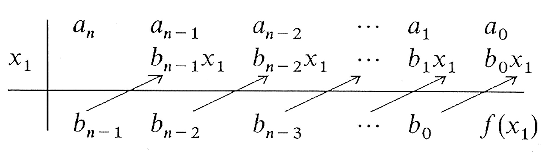
\includegraphics[width=6cm]{./bilder/Hornerschema_1.png}\\
$x_1 \Rightarrow$ Nullstelle (muss erraten werden!!)\\
oberste Zeile = zu zerlegendes Polynom
\end{minipage}
\begin{minipage}[t]{9cm}
\textbf{Beispiel:}\\
$f(x) = x^3-67x-126$\\
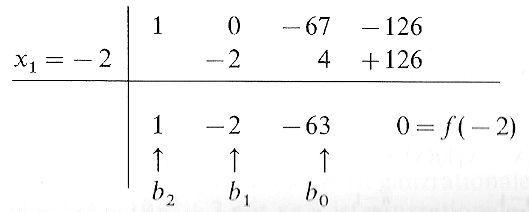
\includegraphics[width=6cm]{./bilder/Hornerschema_2.png}\\
$\Rightarrow f(x) = (x-x_1)(b_2x^2 + b_1x + b_0) = (x+2)(x^2-2x-63)$  
\end{minipage}

\subsection{Lineare Differentialgleichungssysteme erster Ordnung mit konstanten Koeffizienten}
\begin{tabular}{ll}
\textbf{Form:}&
$\begin{array}{l}{\dot{x}=a x+b y+f(t)} \\ {\dot{y}=c x+d y+g(t)}\end{array}=\left(\begin{array}{c}{\dot{x}} \\ {\dot{y}}\end{array}\right)=\left(\begin{array}{ll}{a} & {b} \\ {c} & {d}\end{array}\right)\left(\begin{array}{l}{x} \\ {y}\end{array}\right)+\left(\begin{array}{l}{f(t)} \\ {g(t)}\end{array}\right)$\\
\end{tabular}

\begin{tabular}{ll}
\textbf{Allgemeine Lösung ergibt sich aus der DGL:}&
$\underbrace{\ddot{x}-(a+d) \dot{x}+(a d-b c) x=\dot{f}(t)-d f(t)+b g(t)}_{\text { normale DGL 2. Ordnung} \rightarrow \text { nach } x \text { auflösen }}$
\end{tabular}

\begin{tabular}{ll}
\textbf{Anfangsbedienung:}&
$x_{0}\left(t_{0}\right)=x_{0}, \dot{x}_{0}\left(t_{0}\right)=a x_{0}+b y_{0}+f\left(t_{0}\right)$
\end{tabular}

Anordnung beachten! Gesuchte Grösse immer zu oberst (in diesem Fall ist die gesuchte Grösse $x )$
